\documentclass[12pt,oneside,a4paper,english]{article}
\usepackage[T1]{fontenc}
\usepackage[utf8]{inputenc} % Changed from latin2 to utf8 for better compatibility
\usepackage[margin=2.25cm,headheight=26pt,includeheadfoot]{geometry}
\usepackage[english]{babel}
\usepackage{listings}
\usepackage{color}
\usepackage{titlesec}
\usepackage{titling}
\usepackage[framed, numbered]{matlab-prettifier}
\usepackage{changepage}
\usepackage{amsmath}
\usepackage{hyperref}
\usepackage{enumitem}
\usepackage{graphicx}
\usepackage{fancyhdr}
\usepackage{lastpage}
\usepackage{caption}
\usepackage{tocloft}
\usepackage{setspace}
\usepackage{multirow}
\usepackage{titling}
\usepackage{float}
\usepackage{comment}
\usepackage[strings]{underscore}
\usepackage{booktabs}
\usepackage{indentfirst}
\usepackage{lscape}
\usepackage{booktabs,caption}
\usepackage[flushleft]{threeparttable}
\usepackage[english]{nomencl}
\usepackage{xcolor}
\usepackage{lipsum}

% Set up hyperref
\hypersetup{
colorlinks=true,
linkcolor=blue,
filecolor=magenta,
urlcolor=cyan,
pdftitle={Review Of Historical Astronomical Tools},
pdfpagemode=FullScreen,
}

% --- set footer and header ---
\pagestyle{fancy}
\author{}
\fancyhf{}
\lhead{Astronomical Observation History}
% --- Title formatting ---
\title{\textbf{Review Of Historical Astronomical Tools}}
\date{\today}

% --- Fix typo in Aldebaran throughout document ---
\newcommand{\Aldebaran}{Aldebaran}

% --- End of page settings ---
\begin{document}
\maketitle
\begin{abstract}
Review of various historical astronomy tools utilized to track the proper motion of stars and celestial bodies in the night sky. This article focuses on the following:
\begin{itemize}
\item Astrolabes
\item Armillary Spheres
\item Sextants
\end{itemize}
This will also cover some other tools that are not exclusively used in observation, but were used in support of the above tools. This will be a summary with straightforward instructions on how to use these tools in general, these tools rely on the measuring angles from the horizon of various bodies and utilization of reference books.
\end{abstract}
\section{Astronomy's Beginnings: Armillary Sphere and Astrolabes}
Throughout human history, we have gazed at the stars and given meaning to their seemingly random motions in the sky. The stars hold the key to understanding our place in the universe, and our growth in understanding of these stellar bodies represents our growth as a species. The first mechanical models were called Armillary Spheres. 
Ptolemy around 100 AD began to track the stars in the night sky without as much religious reverence and with more rigorous methods. The zodiac constellations were widely understood as "static" constellations that are seen throughout the year in different seasons. This belief and Ptolemy's command of Greco-Roman mathematics and geometry led him to theorize that the earth stood at the center of the universe. The stars and sun were fixed in "heavenly spheres" that spun around the earth.\cite{ptolo1} This was not unique to Ptolemy, and other astronomers of the time also believed this. 

\begin{figure}[H]
    \centering
    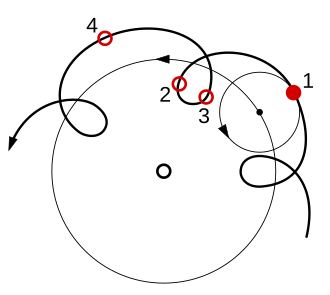
\includegraphics[width=0.5\textwidth]{AstroTools1.png}
    \caption{Path of planet's proper motion that epicycles explained during Ptolemy's Life. From point 1 to point 2, the planet will slow down in the night sky. From 2 to 3, the planet will slow down and then move backwards, and once again accelerate from point 3 to 4. This motion is only visible from the center body (Earth)\cite{ptolopic}}

    \label{fig:epicycles}
\end{figure}
The issue was the fact that the closer bodies (now known as planets) processed backwards and even at times seemed to accelerate across the night sky; the planets seemed to stop, then move backwards, and then accelerate their motion across the sky. These Armillary Spheres were large and difficult to make, so after a few hundred years, 2D astrolabes were introduced and used in government and planning. Astrolabes are models of the night sky generally focused on one hemisphere, gaining accuracy. 

As a consequence, astrolabes relied heavily on reference books and extra parts. The celestial sphere (night sky) is projected over a 2D circle. The base plate represents the 3D sphere, and overtop of it there will be rings that represent the 24-hour cycle. The base plate will have 2 complete circles and flattened ovals; the circles are the Tropic of Cancer and Tropic of Capricorn, and the projection places the south pole at the center of projection. 
On top, a view piece can be aligned with the center of the astrolabe, used for calibrating the instrument and making measurements. Along with many of these astrolabes are highlighted "fixed" heavenly bodies; these are stars that seem to have a consistent location like the zodiac constellations, due to their proximity to the poles. Each projection is unique to each latitude and requires a new plate if the observer moves, so if you want to mark a stellar location of a body via the astrolabe you would do the following:
\begin{itemize}
\item Place the correct baseplate for the latitude the observer is in, hold the astrolabe horizontal with the middle line parallel to the ground.
\item Use the viewing piece to find the zodiac constellation lowest to the horizon.
\item Align the zodiac ring to the matching constellation (or from a reference book).
\item Confirm this is correct by measuring the azimuthal angle (vertical angle) of marked stars or other zodiac constellations.
\item Once completed, while keeping the device horizontal, find a body you would like to mark the location of and align it in the viewfinder or point the rotating top arm. This is the declination angle of the star.
\item You will need a compass; without moving, measure the angle from magnetic north. With the latitude of the observer and these coordinates, astronomers can determine an absolute position of the celestial body. Now the body has a stellar coordinate!
\end{itemize}
In ancient times, these were used mainly for time keeping and astrological predictions. A quadrant (will be expanded upon) could be used with a zodiac calculation book to predict the night sky and tell the observer the dates, these were later referred as an almanac. In this case, the astrolabe would be used as a reference tool. The astrolabe has a notable failure as it doesn't account for the retrograde motion of planets in our solar system. This is why many astronomers had to carry large books, extra plates, and could only use the zodiacs for calibrating the astrolabe. It's worth noting that the astrolabe is relatively simple; Armillary spheres were used in demonstrations of astronomy and in making Astronomical observations. Many astrolabes had the calendar fixed to the ring on the outside of them, so you could use a quadrant to find the declination of a zodiac constellation and thus find the date based on that.
\begin{figure}[H]
\centering
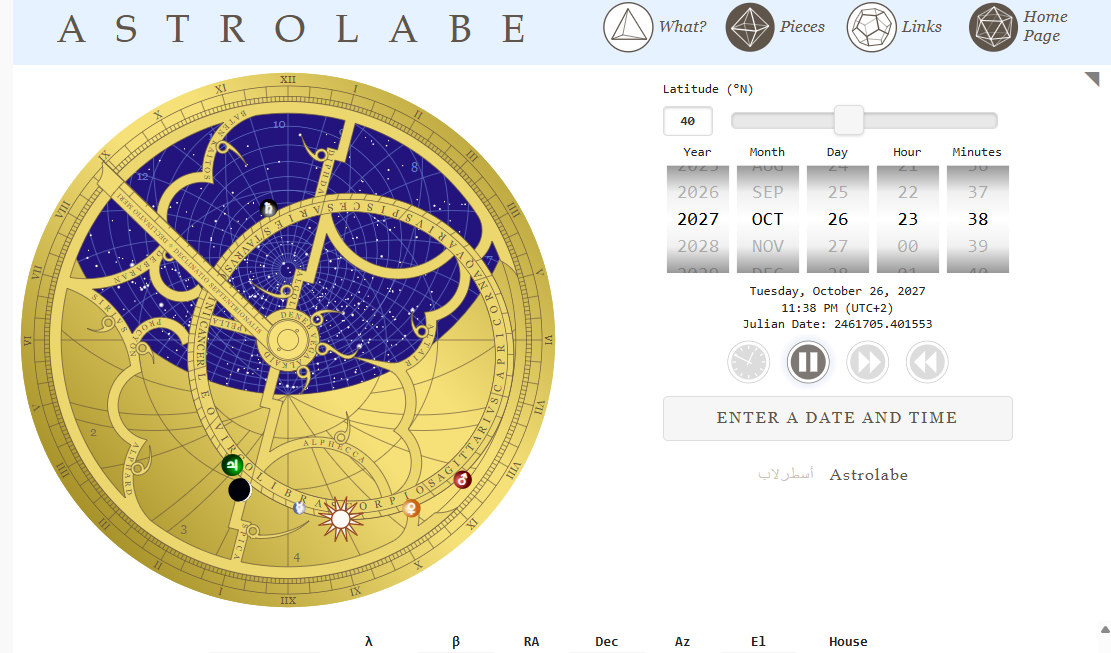
\includegraphics[width=0.8\textwidth]{Astrolaabe1.png}
\caption{Astrolabe demonstration at \href{https://alexboxer.com/astrolabe/}{alexboxer.com}, the astrolabe includes "static bodies" like Aldebaran and Sirius.}
\label{fig:astrolabe}
\end{figure}

Ptolemy said that the planets have their own epicycles, meaning they are moving in small circles while fixed in their heavenly sphere. This explained the motion of every major body in the sky visible at the time, which popularized Ptolemy's Model and Geocentrism as a whole.
\section{Armillary Sphere: Model of Geocentrism}
Armillary Spheres were consistent fixtures in the ancient world as tools for observation of the stars, in line with Ptolemy. Chinese, Indian, and Korean astronomers created their own Armillary Spheres with their own names and slightly different purposes. Some were calendars for tracking seasons and others were for observation alone; these spheres were generally larger, close to the size of 4-5 m. This tool for astronomers represents an outdated tool because of the universe these are modeling, namely Geocentrism. The sphere is generally mounted via a ring around the equator of the sphere. All the spheres rotate freely; the equatorial rotation represents the 24-hour rotation of the day and night. Generally, the sphere is "aligned" or calibrated to the equator and the Zodiac. These celestial landmarks are used to make all nighttime observations by determining the degree difference from these landmarks.
\begin{figure}[H]
\centering
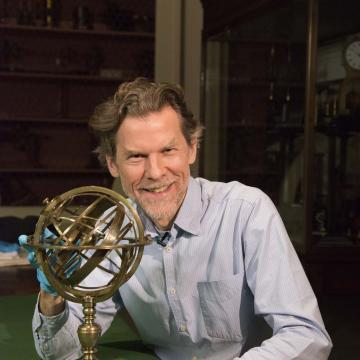
\includegraphics[width=0.5\textwidth]{Sphere1.jpg}
\caption{Photo of Armillary Sphere at Oxford's History of Science Museum.\cite{sphere}}
\label{fig:sphere}
\end{figure}
\section{Mathematics: Quadrants and Astronomy Fundamentals}
As mentioned above, astronomers used landmarks in the night sky to track observations. Some landmarks used are:
\begin{itemize}
\item The Horizon - The equator or horizon of observation.
\item The Zodiac Constellations - These constellations are in the path of the sun and consistently visible.
\item Bright Stars - Consider stars like Polaris; it doesn't move very much over 24 hours, so is always roughly in the same place.
\end{itemize}
The angle from the horizon that a celestial body is becomes very important for determining the motion of these stellar bodies. A Quadrant is a simple and straightforward way of determining the angle of a stellar body from the horizon. There were many quadrants like fixed Mural Quadrants or fixed Quadrants. These were placed on a wall (painted) or fixed on a rotating platform with a telescope fixed to its top. The user could rotate the platform and adjust the azimuth (vertical angle) up to 90 degrees or straight up, thus telling the user the azimuthal angle of the body he or she is observing. This azimuthal angle is still used today by astronomers with more modern methods of measurement. These larger quadrants were designed for use in a fixed latitude or position. As time went on, the Armillary Sphere became out of date and were replaced by models of the heliocentric solar system (known as an orrery). Despite our evolving understanding of the solar system and the stars, the practical math that is required for observation has never really changed. In fact, as the math and concepts became widely understood, smaller quadrants were made for sailors to use when navigating; these were portable and meant to be used with an astrolabe.\cite{quadrant}
\section{Astronomy and Navigation: Sextants and Quadrants}
Astronomy became a matter of industry with the wide adoption of navigating with a sextant. The sextant is the same instrument as a quadrant, but instead of measuring up to 90 degrees, the sextant can measure the distance of two stellar bodies up to 60 degrees. Sextants used other bodies like the sun or stars and measured their distance from the horizon; sailors could quickly take a single measurement and refer to a reference book to quickly find their location while they sailed. Quadrants and telescopes were sometimes designed with filters to look at the sun, but many sextants had this filter so that navigation could be completed during the day. Without getting too far into specifics, the sailor determines the estimated location of the ship by measuring its speed (via counting knots) and using the heading at the last known position. After, the sailor refers to an almanac that will usually give insight into what celestial body the sailor should use. An astrolabe could be utilized instead to determine the best celestial body to use. He or she would observe the angle of the body above the horizon and referencing the reference chart or astrolabe to find the latitude the ship is located in, then the ship's true location is know known and noted, this will be used to estimate the next measurement to make and is written in a navigation log.\cite{sext}
\section{Conclusion}
The Armillary Sphere is the first mechanical model of the night sky and eventually allowed for the creation of the astrolabe, letting many people utilize stellar observation in timekeeping and navigation. The tools were paired with observational mathematics that are easy to reproduce, allowing us to look back into the past and see what the night sky looked like in ancient times and even apply modern methods to these measurements. Modern databases like SIMBAD have historical records from medieval times because of this.
\newpage
\section{References}
\bibliography{AstroTools.bib}
\bibliographystyle{ieeetr}
\end{document}